\documentclass{article}
\usepackage{graphicx} % Required for inserting images
\usepackage{listings}
\usepackage{url} % Add the url package
\usepackage{titlesec}

\documentclass{article}
\usepackage{graphicx} % Required for inserting images


\usepackage{titlesec}

\title{ECS171 Group 8 Report}
\author{Boquan Fang, Sage Deo, Ishita Dutta, Zhuo Chen}
\date{June 2023}
% \url{https://github.com/BoquanFang/ECS171_Term_Project.git}



\maketitle

\begin{document}

\section{Introduction}
Listening to music is a popular activity that people all over the world engage in. 
Everyone has their own music taste and their own way of listening to music.
Some people exclusively listen to music by picking a single album by a single artist 
and listening to it from beginning to end, but others curate playlists of music from
various albums by various artists. These playlists are often designed to suit specific
moods or feelings, and it is important to the listening experience that the contents of
each playlist is internally consistent to avoid jarring the listener or inducing whiplash.

Prior to the creation of intelligent recommender systems such as those employed by 
Spotify and YouTube Music, humans would create playlists for themselves or for others,
and thus would seleect songs for each playlist that both fit that playlist's desired mood
and are tonally similar to the other songs on the playlist. However, as such 
online music platforms emerged, they became ways of exploring new types of music cheaply.
Users did not have to spend money on physical media or digital rights to a song that they
might not enjoy, so they could listen to lots of music themselves to determine if they liked it
or not. Later, as content recommendation algorithms became stronger and amassed more data
to train on, automatic recommendation methods became a viable way for users of these platforms
to find new music to listen to without having to listen to all the songs themselves. 

Thus, the problem of this research paper is about determining whether a chosen song is similar enough
to others in a given playlist to be accepted into that playlist. This can be used to recommend
new songs to the user based on the contents of their existing playlists; users are more likely
to enjoy songs that can fit into their existing playlists, especially those they listen to most.
Additionally, it can be used to generate entirely new playlists for users, starting from a small
playlist of a few of their favorite songs, and then repeatedly searching for and adding songs that
fit the energy of the newly-generated playlist. This creates completely new full-sized playlists 
with consistent energy and tone and potentially new songs that the user has not listened to before.
This will create a novel but still enjoyable listening experience. 

\section{Literature Review}
Some study has been done on Spotify data. For example, Nijkamp et al. used the Spotify API
to investigate whether a song's popularity could be predicted based on its other features, and found
that it could not. Pareek et al. also found that a random forest model could classify songs
as popular or unpopular with an accuracy of 86\%. Code AI managed to predict popularity with a KNN
model with an error of only 0.03\%. However, all of these studies are addressing the problem
of predicting popularity; there is currently a gap in knowledge surrounding the problem of fitting
songs into playlists. 

One instance of using machine learning to recommend songs rather than predict their popularity is
Alexander Bricken's Gaussian Mixture model which recommend songs based on their Spotify API
features. Though this is not exactly the same as determining whether a song fits into a playlist,
it is similar and a useful starting point.

\section{Dataset Description and Exploratory Data Analysis of the Dataset}
This project’s dataset is retrieved by the user level interface from the Spotify developer API. With two given URL to a playlist and a song, the user level interface could access the Spotify developer API and save the data for both the playlist and the given song in a CSV file. The number of rows is depended on how many songs that a given playlist has. The Spotify developer API provides thirteen attributes for a given song: name, danceability, energy, key, loudness, mode, speechiness, acousticness, instrumentalness, liveness, valence, tempo, and duration. The name represents the name of a given song and that would not be considered in our exploratory data analysis part. Danceability “describes how suitable a track is for dancing based on a combination of musical elements including tempo, rhythm stability, beat strength, and overall regularity.” Energy represents “is a measure from 0.0 to 1.0 and represents a perceptual measure of intensity and activity.” Key represents the track that a given music is in. Loudness shows the overall loudness of a song in decibels.  Mode indicates “the modality (major or minor) of a track, the type of scale from which its melodic content is derived”. Speechiness indicates the presence of oral spoken words in the given song. Acousticness is the confidence interval of the track in terms of acoustic. Instrumentalness “predicts whether a track contains no vocals.” Liveness detects “the presence of an audience in the recording.” Valence is “a measure from 0.0 to 1.0 describing the musical positiveness conveyed by a track.” Temp covers “the overall estimated tempo of a track in beats per minute (BPM).” The attributes duration indicates the duration of the songs in millisecond. 
The attributes energy is the most important attribute, since we will use the energy attribute as an indicator of whether the given song fits well with the playlist. Therefore, exploratory analysis needs to generate a correlation heat and analyze the correlation between every attribute with respect to the energy attribute. The group determines that every attribute which has a correlation that less than 0.2 in absolute value should not be included in the final training set. If those attributes are included in the training set, those attributes will generate noise and overfit the model.

\section{Proposed Methodology}


\section{Experimental Results}

\section{Interface Design}
\maketitle
\subsection{Interface Introduction}
Once we have developed the model, we should use Flask to create an API that allows users to input a playlist and get the desired results. Flask is a popular Python web framework that is suitable for building lightweight web applications and APIs.
\begin{lstlisting}[language=Python]
# You can use this command to install the flask
pip install flask
\end{lstlisting}


\subsection{User Interface}
To create a website using Flask that allows users to input a playlist URL and extract its attributes, you'll need to perform the following steps:
1. Get an access token for the Spotify Web API:
You should first Register a new application on the Spotify Developer Dashboard (https://developer.spotify.com/dashboard/applications).
Obtain the client ID and client secret and then get the access token.
2. Use the access token to get the playlist data.
3. Get the song names and audio features from the playlist data
4. Creating a text box for a user to enter a single song's URL and retrieve its data.
5. Run the model on the page that we open, and get all the results based on our training model(the Traning dataset is the whole playlist, the test dataset is the song that we enter.


\subsection{API: Get the song names and audio features from the playlist data}
You should first make a get request to the API URL. Then, parse the response to retrieve the relevant information. The response will include an array of track objects, each containing various details about the track. I will show the code below since this part might be difficult to understand.
\begin{lstlisting}[language=Python]
# Python code snippet
    api_url = f'https://api.spotify.com/v1/playlists/{playlist_id}/tracks'
    headers = {'Authorization': f'Bearer {access_token}'}
    response = requests.get(api_url, headers=headers)
    response_data = response.json()

    # Get the song names and audio features from the playlist data
    song_names = []
    audio_features = []
    sp = spotipy.Spotify(auth=access_token)
    for item in response_data['items']:
        track_uri = item['track']['uri']
        track_name = item['track']['name']
        song_names.append(track_name)
        audio_features.append(sp.audio_features(track_uri)[0])

\end{lstlisting}
To accomplish the tasks you mentioned, we need to create four HTML files: index.html, music.html, song.html, and songs.html.

index.html: This file will serve as the welcome page where users can enter the playlist URL. It should contain necessary HTML elements such as input fields, buttons, and a form to gather user input.

music.html: This file will include essential code for integrating with the Spotify API or any other music-related functionality you're implementing. 

songs.html: This file is essential for displaying song attributes and allowing users to select a single song as a test case. It should include HTML elements to show song details such as title, artist, album, and other relevant information.

song.html: This file will display detailed information about a single song, including its attributes and several graphs to support your model. Additionally, it can include the final test result to assess the performance of your model. It uses HTML elements like headings, paragraphs, charts, or visualizations to present the information effectively.
% \subsection{Figure 1}
\begin{figure}[h]
\centering
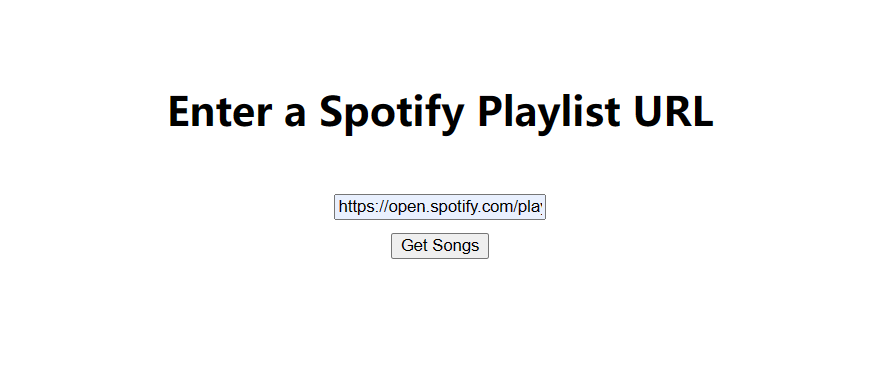
\includegraphics[width=1\textwidth]{1.png}
\caption{This is the welcome page of the user interface}
The user could enter any playlist URL here.
\label{fig:enter-label}
\end{figure}
\begin{figure}[h]
\centering
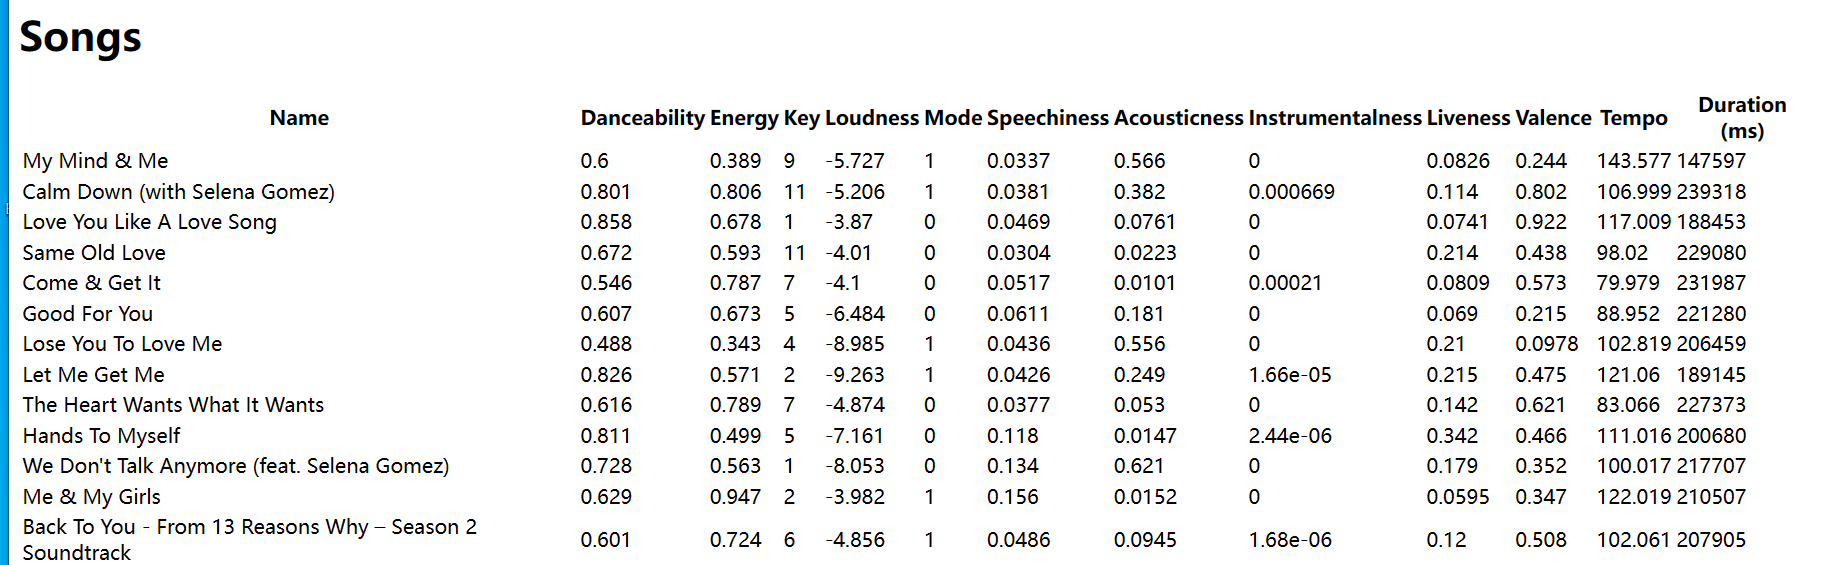
\includegraphics[width=1\textwidth]{2.png}
\caption{This is the attribute that we extract from the playlist.}
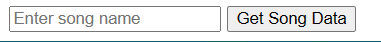
\includegraphics[width=0.5\textwidth]{3.png}
\caption{The user can enter any song's URL as the test dataset here.}
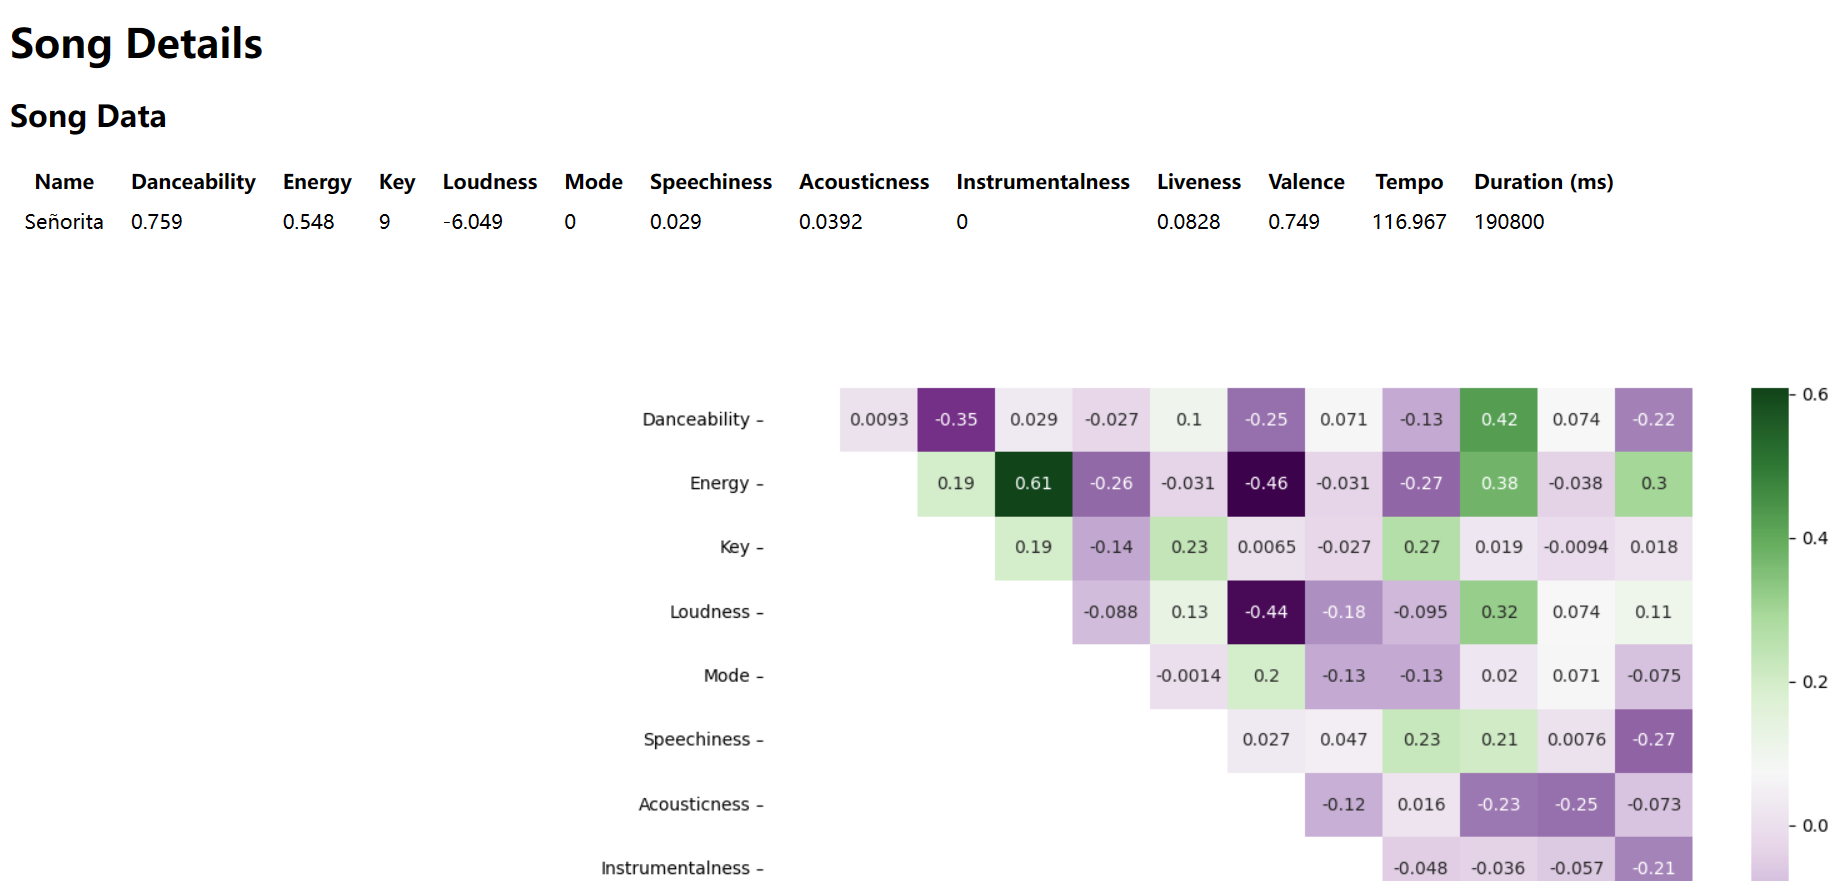
\includegraphics[width=1\textwidth]{4.png}
\caption{Here is a new page after the user enters the song's URL, and we can see the attributes of this song.}
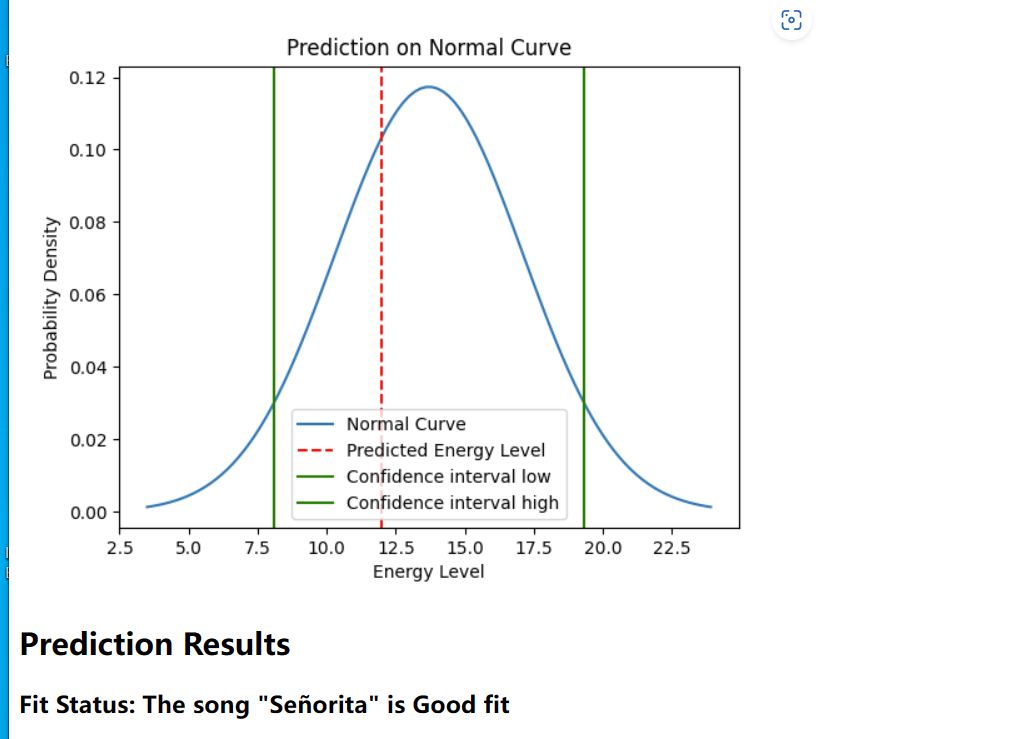
\includegraphics[width=1\textwidth]{5.png}
\caption{Finally, it shows the result at the bottom of the page about whether this song's style is similar to our playlist.}
\label{fig:enter-label}
\end{figure}
\clearpage
\section{Conclusion and Discussion}

\end{document}
